\chapter{Examples} \label{sec:examples}

\section{Short Tutorial}

In this section, we write a driver code which calls the Mesquite
library to improve the quality of a test mesh. This tutorial section
is aimed at giving the user a feel for Mesquite: \emph{this section is not
where to look for detailed information}. In particular, information
pertaining to loading a particular mesh format (see Chapter \ref{sec:meshes}), 
interacting through a particular mesh interface (section \ref{sec:MeshData}), 
and details of defining geometric domains (see Chapter \ref{sec:geom}) are not
given in this section.

First, we write a small program using Mesquite's simplified API, or
wrappers, to show the fastest way to deploy Mesquite functionality to
improve a mesh.  The wrapper concept, as well as details about the
different wrappers available, are described in section
\ref{sec:tutWrapper}.  Following this first example, we set up customized mesh
improvement tool using Mesquite's low-level API, the details of which
are described in section \ref{sec:tutDetailedAPI}.

\subsection{Tutorial File Template}
\label{sec:tutfile}

To create and link a driver code, the Mesquite library must be
installed per the instructions of section \ref{sec:compiling}. 
The commands and file names specified in this section are relative 
to the installed \texttt{testsuite/tutorial} directory.  It 
is assumed that that is the working diretory.
This tutorial begins with the file \texttt{tutorial.cpp}, 
which contains the following template:
\begin{verbatim}
1.  #include "Mesquite_all_headers.hpp"
    #include <ostream>
2.  using namespace Mesquite;
    int main(int argc, char* argv[])
    {
3.    MsqError err;

      if (argc != 2) {
        std::cerr << "Expected mesh file names as single argument."
                  << std::endl;
        exit (EXIT_FAILURE);
      }

      // new code starts here
4.    //... 

      return 0;
    }
\end{verbatim}
The lines labeled 1-3 highlight three basic aspects of using Mesquite;
\begin{enumerate}
\item For convenience, Mesquite provides the header file
\begin{center}
\texttt{include/Mesquite\_all\_headers.hpp}
\end{center} which includes all Mesquite
headers. Although this is the easiest way to handle the include directives,
it may slow down compilation of the application.  
\item All Mesquite classes are part of the \texttt{Mesquite} namespace. 

\item  The \texttt{MsqError} class defines an object type used to communicate
Mesquite errors to the application.  The calling application must pass
an instance of the \texttt{MsqError} class or an instance of a subclass of
\texttt{MsqError} to many Mesquite functions.  The state of the error object
may be checked by casting the instance ot a Boolean or using it in a 
Boolean context.  The state is cleared by calling the \texttt{clear} method.
\item In the sections that follow, we guide the user through the steps
necessary to smooth a mesh using Mesquite.  All new lines of code to be
added to the template file start in this position and are added in the order
in which they are discussed.
\end{enumerate}

The code above takes a mesh file name as a command line argument and
performs no action. We can compile it in the 
(\texttt{examples/}) directory with the command:

\begin{verbatim}
                        make -f tutorial.make
\end{verbatim}


\subsection{Loading a Test Mesh}
\label{sec:tutMesh}
Our next step is to load one of the test meshes distributed with
Mesquite.  These meshes are distributed in the VTK unstructured mesh
format, the details of which are given in \cite{VTKbook, VTKuml}. This
format was chosen because of its readability and ease of use. 
In this tutorial we use
the simplest mechanism for loadling a mesh into Mesquite; different
options are described in Chapter \ref{sec:meshes}.  In particular, to
load a VTK test mesh in Mesquite, instantiate the Mesquite mesh
database object,
\texttt{MeshImpl}, and use the \texttt{read\_vtk} member function by
adding the following lines to the file template described in
\ref{sec:tutfile}.
\begin{verbatim}
  Mesquite::MeshImpl my_mesh;
  my_mesh.read_vtk(argv[1], err); 
  if (err) 
  {
    std::cout << err << std::endl;
    return 1;
  }
\end{verbatim}

If the mesh read in contains more than one type of element, Mesquite will automatically
handle the mixed elements with no additional effort required.

Mesquite also provides a function to write a mesh
file in VTK format, given a \texttt{MeshImpl} object:
\begin{verbatim}
  my_mesh.write_vtk("original_mesh.vtk",err); 
\end{verbatim}

Mesquite deals automatically with all types of supported elements 
(triangles, quadrilaterals, tetrahedra, hexahedra, wedges, and pyramids),
and also hybrid meshes consisting of mixed element types.  
Some meshes require geometry information as well.  When improving a surface mesh, Mesquite must be provided information
about surface(s) the mesh is constrained to lie on and the association between
mesh entities and entities of the geometric domain (surfaces, curves, etc.)
Because Mesquite is inherently a 3D code, all 2D meshes must specify some
geometry constraints.  The details
for general geometric surfaces are explained in Chapter 
\ref{sec:geom}. In this section,
we show how to define the geometry of a 2D planar mesh, specified by a
point $(x,y,z)$ and a normal. For example, the following defines an xy-plane
shifted five units in the z-direction:
\begin{verbatim}
  Vector3D normal(0,0,1);
  Vector3D point(0,0,5);
  PlanarDomain my_mesh_plane(normal, point);
\end{verbatim}


\subsection{Improving the Mesh with a Wrapper Class}
\label{sec:tutWrapper}
The simplest way to use a Mesquite mesh quality improvement
procedure is to instantiate one of the wrapper classes described in Chapter 
\ref{sec:wrappers}. Here, we will instantiate the
\texttt{ShapeImprovement} wrapper and use it to improve 
the Mesh we created earlier.  Mesquite can optimize the mesh
without further input from the user by utilizing preset, default
values.  If some customization is desired, the wrapper classes also
allow users to set the most important parameters of the underlying
algorithms and metrics (see Chapter 
\ref{sec:wrappers} for details).
\begin{verbatim}
Mesquite::ShapeImprover mesh_quality_algorithm;
mesh_quality_algorithm.run_instructions(&my_mesh,
                                        &my_mesh_plane,  err);
//Should check the error object after the instruction is ran
// to see whether the instructions were all successful.
if (err) 
{
    std::cout << err << std::endl;
    return 1;
}
\end{verbatim}

Once the algorithm has been executed using the {\tt run\_instructions} member
function of the wrapper class, the improved mesh can be written to a new
file:
\begin{verbatim}
  my_mesh.write_vtk("smoothed_mesh.vtk",err); 
\end{verbatim}
This completes the code necessary for the simple wrapper example.  Once
the code has successfully compiled by typing the {\tt make} command given in
section \ref{sec:tutfile}, 
run it from the tutorial directory \texttt{mesquite/testSuite/tutorial/}
with a mesh file name as a command line 
argument by typing 
\begin{verbatim}
./tutorial ../../meshFiles/2D/VTK/square_quad_10_rand.vtk
\end{verbatim}
The code creates the files original\_mesh.vtk
and improved\_mesh.vtk in the current directory.  These two meshes, the
original and the optimized, are
shown in figure \ref{fig:square_rand}.  The text output of the code,
shown below, reports the inverse mean ratio quality metric statistics for
the mesh at three stages:  the original mesh, the mesh at an intermediate
step of the optimization, and the final mesh.  The optimized mesh consists
of square quadrilaterals which have an inverse mean ratio value of 1.0.
\begin{verbatim}
************** QualityAssessor Summary **************

  There were no inverted elements detected. 
  No entities had undefined values for any computed metric.

             metric    minimum    average        rms    maximum
 Inverse Mean Ratio    1.01013    1.16655     1.1738    1.79134

************** QualityAssessor Summary **************

  There were no inverted elements detected. 
  No entities had undefined values for any computed metric.

             metric    minimum    average        rms    maximum
 Inverse Mean Ratio    1.01013    1.16655     1.1738    1.79134

************** QualityAssessor Summary **************

  There were no inverted elements detected. 
  No entities had undefined values for any computed metric.

             metric    minimum    average        rms    maximum
 Inverse Mean Ratio          1          1          1          1
\end{verbatim}
\begin{figure*}[htbp]
\begin{center}
    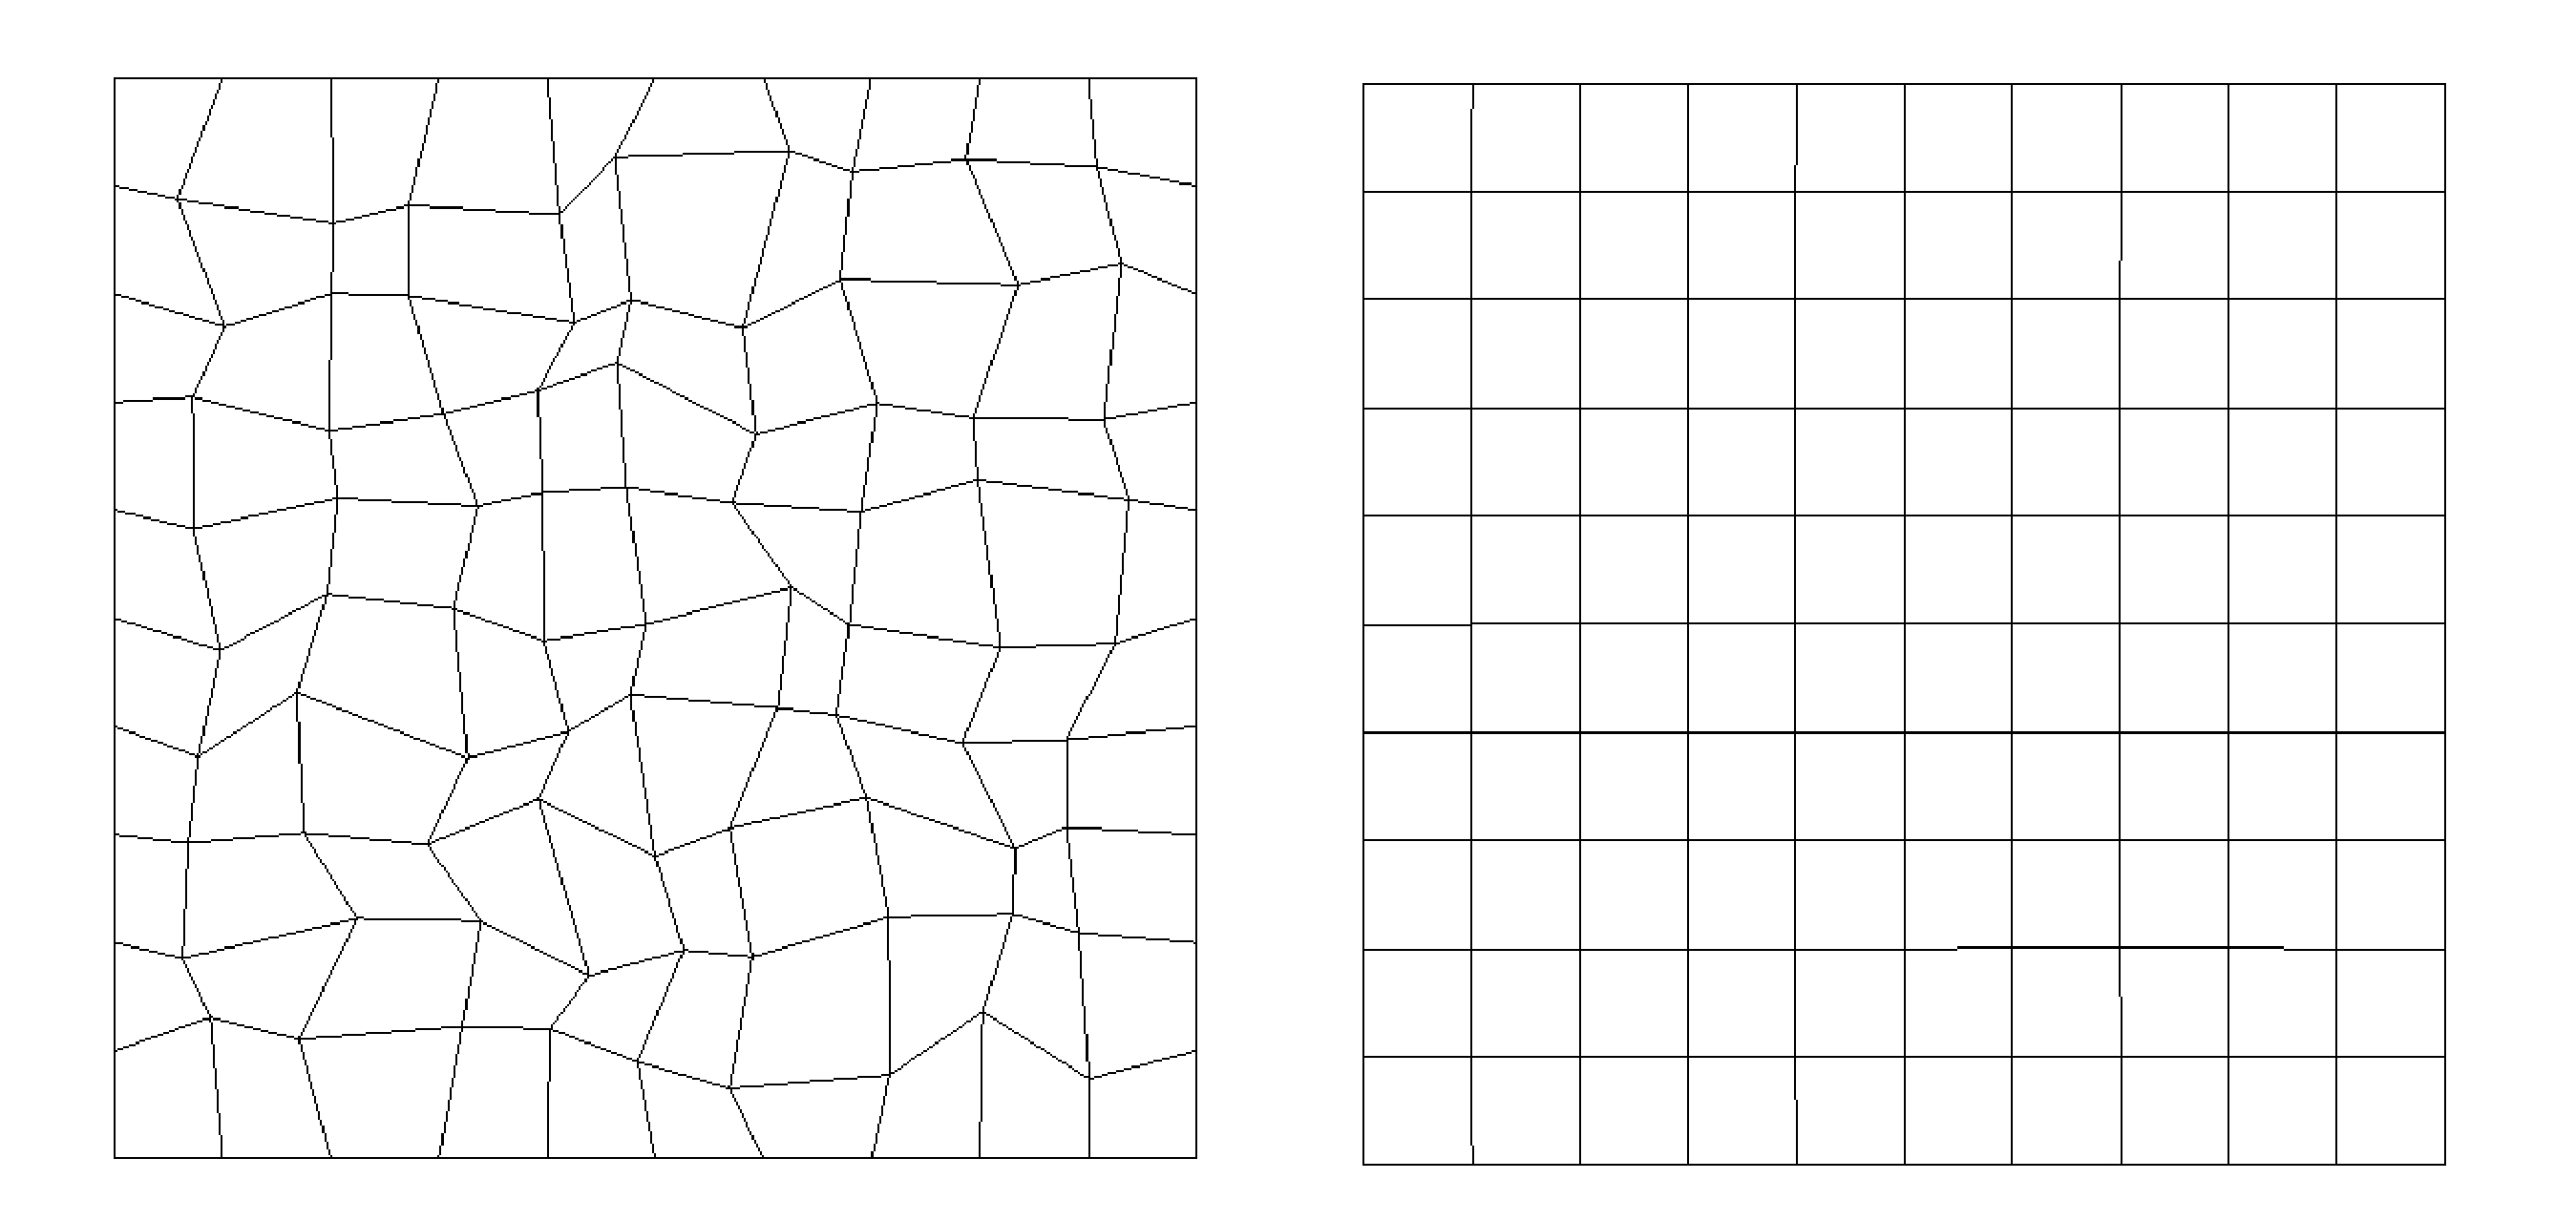
\includegraphics[height=50mm]{square_rand.eps}
    \caption{square\_quad\_10\_rand.vtk mesh. The original mesh is on the left, the mesh smoothed with \texttt{ShapeImprover} is shown on the right.}
    \label{fig:square_rand}
\end{center}
\end{figure*}


\subsection{Improving the Mesh with the Low Level API}
\label{sec:tutDetailedAPI}
If the user requires in-depth control over the mesh quality improvement
process, the use of lower-level Mesquite classes provides an extensive
amount of flexibility.   In particular, the user can specify the quality
metric, objective function template, and optimization algorithm by
instantiating particular instances of each.  For each, various options
such as numerical or analytical gradient and Hessian evaluations or
the patch size can be selected.  Furthermore, the user can fine tune
the optimization algorithm performance by creating and setting the parameters 
of the termination criteria.
%for both inner and outer iterations.
%mbrewer removed reference to inner and outer iterations.
%{\tt LAF have we talked about inner and outer iterations before? perhaps
%too advanced for the tutorial}

Once these core objects have been created and customized, the user
creates an instruction queue and adds one or more quality improvers
and quality assessors to it.  The mesh optimization process is initiated
with the {\tt run\_instructions} method on the instruction queue
class.

In this section, we provide a simple example to highlight the main
steps needed for this approach.  The code segment given below performs
the same functionality as the wrapper class highlighted in the
previous section.  The comment lines provide high level documentation;
the details of each class and the low-level API are not described here.
%extensively treated in Section 
%\ref{sec:detailedAPI}.

\begin{verbatim}
    // creates a mean ratio quality metric ...
  IdealWeightInverseMeanRatio inverse_mean_ratio(err);

    // sets the objective function template
  LPtoPTemplate obj_func(&inverse_mean_ratio, 2, err);
  
    // creates the optimization procedures
  TrustRegion t_region(&obj_func);

    //performs optimization globally
  t_region.use_global_patch(); 

    // creates a termination criterion and 
    // add it to the optimization procedure
    // outer loop: default behavior: 1 iteration
    // inner loop: stop if gradient norm < eps
  TerminationCriterion tc_inner;
  tc_inner.add_absolute_gradient_L2_norm( 1e-4 ); 
  t_region.set_inner_termination_criterion(&tc_inner);

    // creates a quality assessor
  QualityAssessor m_ratio_qa(&inverse_mean_ratio);
    // creates an instruction queue
  InstructionQueue queue;
  queue.add_quality_assessor(&m_ratio_qa, err); 
  queue.set_master_quality_improver(&t_region, err); 
  queue.add_quality_assessor(&m_ratio_qa, err); 

    // do optimization of the mesh_set
  queue.run_instructions(&my_mesh, &my_mesh_plane, err); 
  if (err) {
    std::cout << err << std::endl;
    return 2;
  }
\end{verbatim} 

\subsection{Mesh Improvement Examples}

The left image in figure \ref{fig:hole} shows a mesh that has
been degraded by moving the disk from the right side of the square to
the left while keeping the mesh topology fixed.
The mesh file
\newline
\texttt{mesquite/meshFiles/2D/VTK/hole\_in\_square.vtk} contains the
information for this mesh.  If you plan to run this example, note that
the normal direction that defines the geometry is now $(0,0,-1)$.
This change must be made in the tutorial example code
as was done in section \ref{sec:tutMesh}, or an error message will be
thrown.
\begin{verbatim}
  Vector3D normal(0,0,-1);
  Vector3D point(0,0,-5);
  PlanarDomain my_mesh_plane(normal, point);
\end{verbatim}

We can now improve the mesh with the wrapper mentioned in
\ref{sec:tutWrapper} or the detailed API mentioned in
\ref{sec:tutDetailedAPI}. 
Because we changed the normal, the driver code must be recompiled;
otherwise the code and executable are as before.
Once the code is recompiled, type 
\begin{verbatim}
./tutorial ../../meshFiles/2D/VTK/hole_in_square.vtk
\end{verbatim}
to improve this mesh.
The smoothed mesh is shown in the right image of figure
\ref{fig:hole}.
The vertex locations have been repositioned and significantly improve
the quality of the mesh, as shown by the onscreen
quality assessor output:  
\begin{verbatim}
************** QualityAssessor(free only) Summary **************

  Evaluating quality for 140 elements.
  This mesh had 140 quadrilateral elements.
  There were no inverted elements detected. 
  No entities had undefined values for any computed metric.

            metric     minimum     average         rms     maximum    std.dev.
Inverse Mean Ratio     1.07588     85.8391     463.357     5037.46     455.336

************** QualityAssessor(free only) Summary **************

  Evaluating quality for 140 elements.
  This mesh had 140 quadrilateral elements.
  There were no inverted elements detected. 
  No entities had undefined values for any computed metric.

            metric     minimum     average         rms     maximum    std.dev.
Inverse Mean Ratio     1.01896     1.83479     1.91775     3.36336    0.557969
\end{verbatim}
\begin{figure*}[htbp]
\begin{center}
    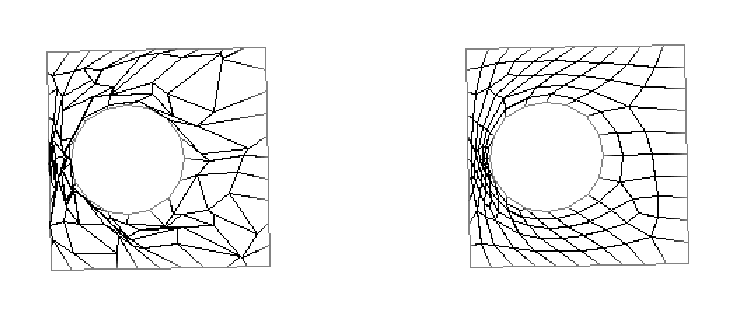
\includegraphics{hole_in_square.ps}
    \caption{hole\_in\_square.vtk mesh. The original mesh is on the left, the mesh smoothed with
    Mesquite is shown on the right.}
    \label{fig:hole}
\end{center}
\end{figure*}


%%... section on testing ...

\subsection{Regression Testing}
\label{sec:RegressionTesting}
Regression testing encompasses
running unit tests as well as comparing results data against "blessed"
or "gold" data.  An example of comparing results of a smoothed mesh
against a gold version is in
\texttt{mesquite/testSuite/parallel\_smooth\_laplace/par\_hex\_smooth\_laplace.cpp}.
This utilizes a function in \texttt{MeshUtil}, \texttt{meshes\_are\_different}, to compare
two \texttt{MeshImpl} objects (within a specified numerical tolerance).  It is
recommended that both unit testing and gold-comparison testing be
included in your test code development.
